\section{System Design}\label{secdesign}

Throughout the development life cycle there were a number of changes regarding technologies and overall design of the web application. Having initially intended to follow the architecture detailed in \textit{Figure \ref{initarchitecture}}, a number of problems and events ultimately led to some changes.

The restructuring of this application was not major but did greatly benefit the project, seeing the addition of new technologies and removal of those that were deemed unnecessary. In this section, the overall design of the web application will be explained under the following headings; \textit{Web Application}, \textit{Currency Data}, and \textit{Machine Learning}.

\subsection{Web Application}

Flask Blueprints \cite{flaskblueprints} are adopted in this web application to organise and separate distinct components or modules, in this case the client and the \textit{Application Programming Interface} or API. Blueprints define a collection of behaviours, views, templates, and static files which can be then used anywhere in the application. Although this project does not intend to take advantage of the reusability of blueprint modules, it will benefit from the elegant architectural structure that can be achieved with them. 

The application consists of two separate blueprints registered to the following URL sub-domains: \mintinline{python}{""} and \mintinline{python}{"/api"}. The client has the responsibility of serving the HTML files to the user and can be accessed as such: \textcolor{NavyBlue}{\url{https://currencyanalyser.herokuapp.com/}}. The client has one route, \mintinline{python}{"/"}, that returns the single page web application, in the form of the index.html file that links the built and minified Vue.js code via a script tag. The single page web application consists of the following pages:

\begin{itemize}
    \item \textit{Home:} This is the root page, containing the application title. Page URL: \textcolor{NavyBlue}{\url{https://currencyanalyser.herokuapp.com/}}
    \item \textit{Dashboard:} This is the main page of the application, displaying a collection of cards containing prices and rates of various currencies, along with machine learning predictions of Bitcoin prices. Cards containing graphs were originally going to be rendered using the D3.js library, a fantastic data-driven approach to Document Object Model manipulation. However, D3.js was unnecessarily sophisticated for its use being solely to create dynamic graphs. Chart.js is a simple but powerful data visualisation library, that serves the purposes of this project perfectly. Page URL: \textcolor{NavyBlue}{\url{https://currencyanalyser.herokuapp.com/#/dashboard}}
    \item \textit{About:} This simple "About" page contains details relating to the team, context of the project and contact details. Page URL:\\ \textcolor{NavyBlue}{\url{https://currencyanalyser.herokuapp.com/#/about}}
    \item \textit{Error:} This is a standard error page which displays when any URL containing a domain which is not mentioned above is queried. Page URL: \textcolor{NavyBlue}{\url{https://currencyanalyser.herokuapp.com/#/some\_invalid\_url}}.
\end{itemize}

The project's API has the responsibility of returning machine learning and currency data and can be accessed via \textcolor{NavyBlue}{\url{https://currencyanalyser.herokuapp.com/api/}}. The API blueprint utilises the Flask-RESTful extension, adhering to the standard architectural design for web services and web APIs.

\subsection{Currency Data}
The project's API populates data to be returned through the use of background workers, which are used to pull data at scheduled intervals of $n$ seconds. These workers also pull data of $n$ days to train the machine learning model with the previous days result, and to predict the end price for the current day. Initially, the API was to act as the database handler or \textit{DAO (Data Access Object)}, controlling and encapsulating actual communications to MongoDB. The scripts would publish the new values and the API listener threads would handle the data received. 

However, during the implementation of this concept for handling data, we came upon the realisation that the API would be dealing unnecessarily with MongoDB. The web application only deals with the most recent data, and thus can be optimised by pre-formatting any data to suit the web application's requirements. The data from the API is requested and refreshed by the web application constantly for the most recent currency data. Consequentially, it would be cumbersome to query the MongoDB database and reformat the query result with every request. The scripts were already communicating with the API via Redis, thus it seemed optimal that the scripts handle MongoDB and use Redis solely to share the most recent data with the API. This would subsequently simplify the code and reduce the dependencies the scripts have on one another, e.g. the worker relies on the web application to save the data published, or the worker needs to be ran to allow a clean shutdown of the web application. The web application's Heroku CPU allocation is no longer competing with listener threads, and the management of MongoDB will be abstracted from the API rather than delegated to it. 

Furthermore, as the machine learning implementation developed we realised it would no longer require the live currency data, meaning it was no longer necessary to save real time currency data to the MongoDB database. Now this data will solely be used for live currency data displayed on web application.

\begin{figure}[h]
    \centering
    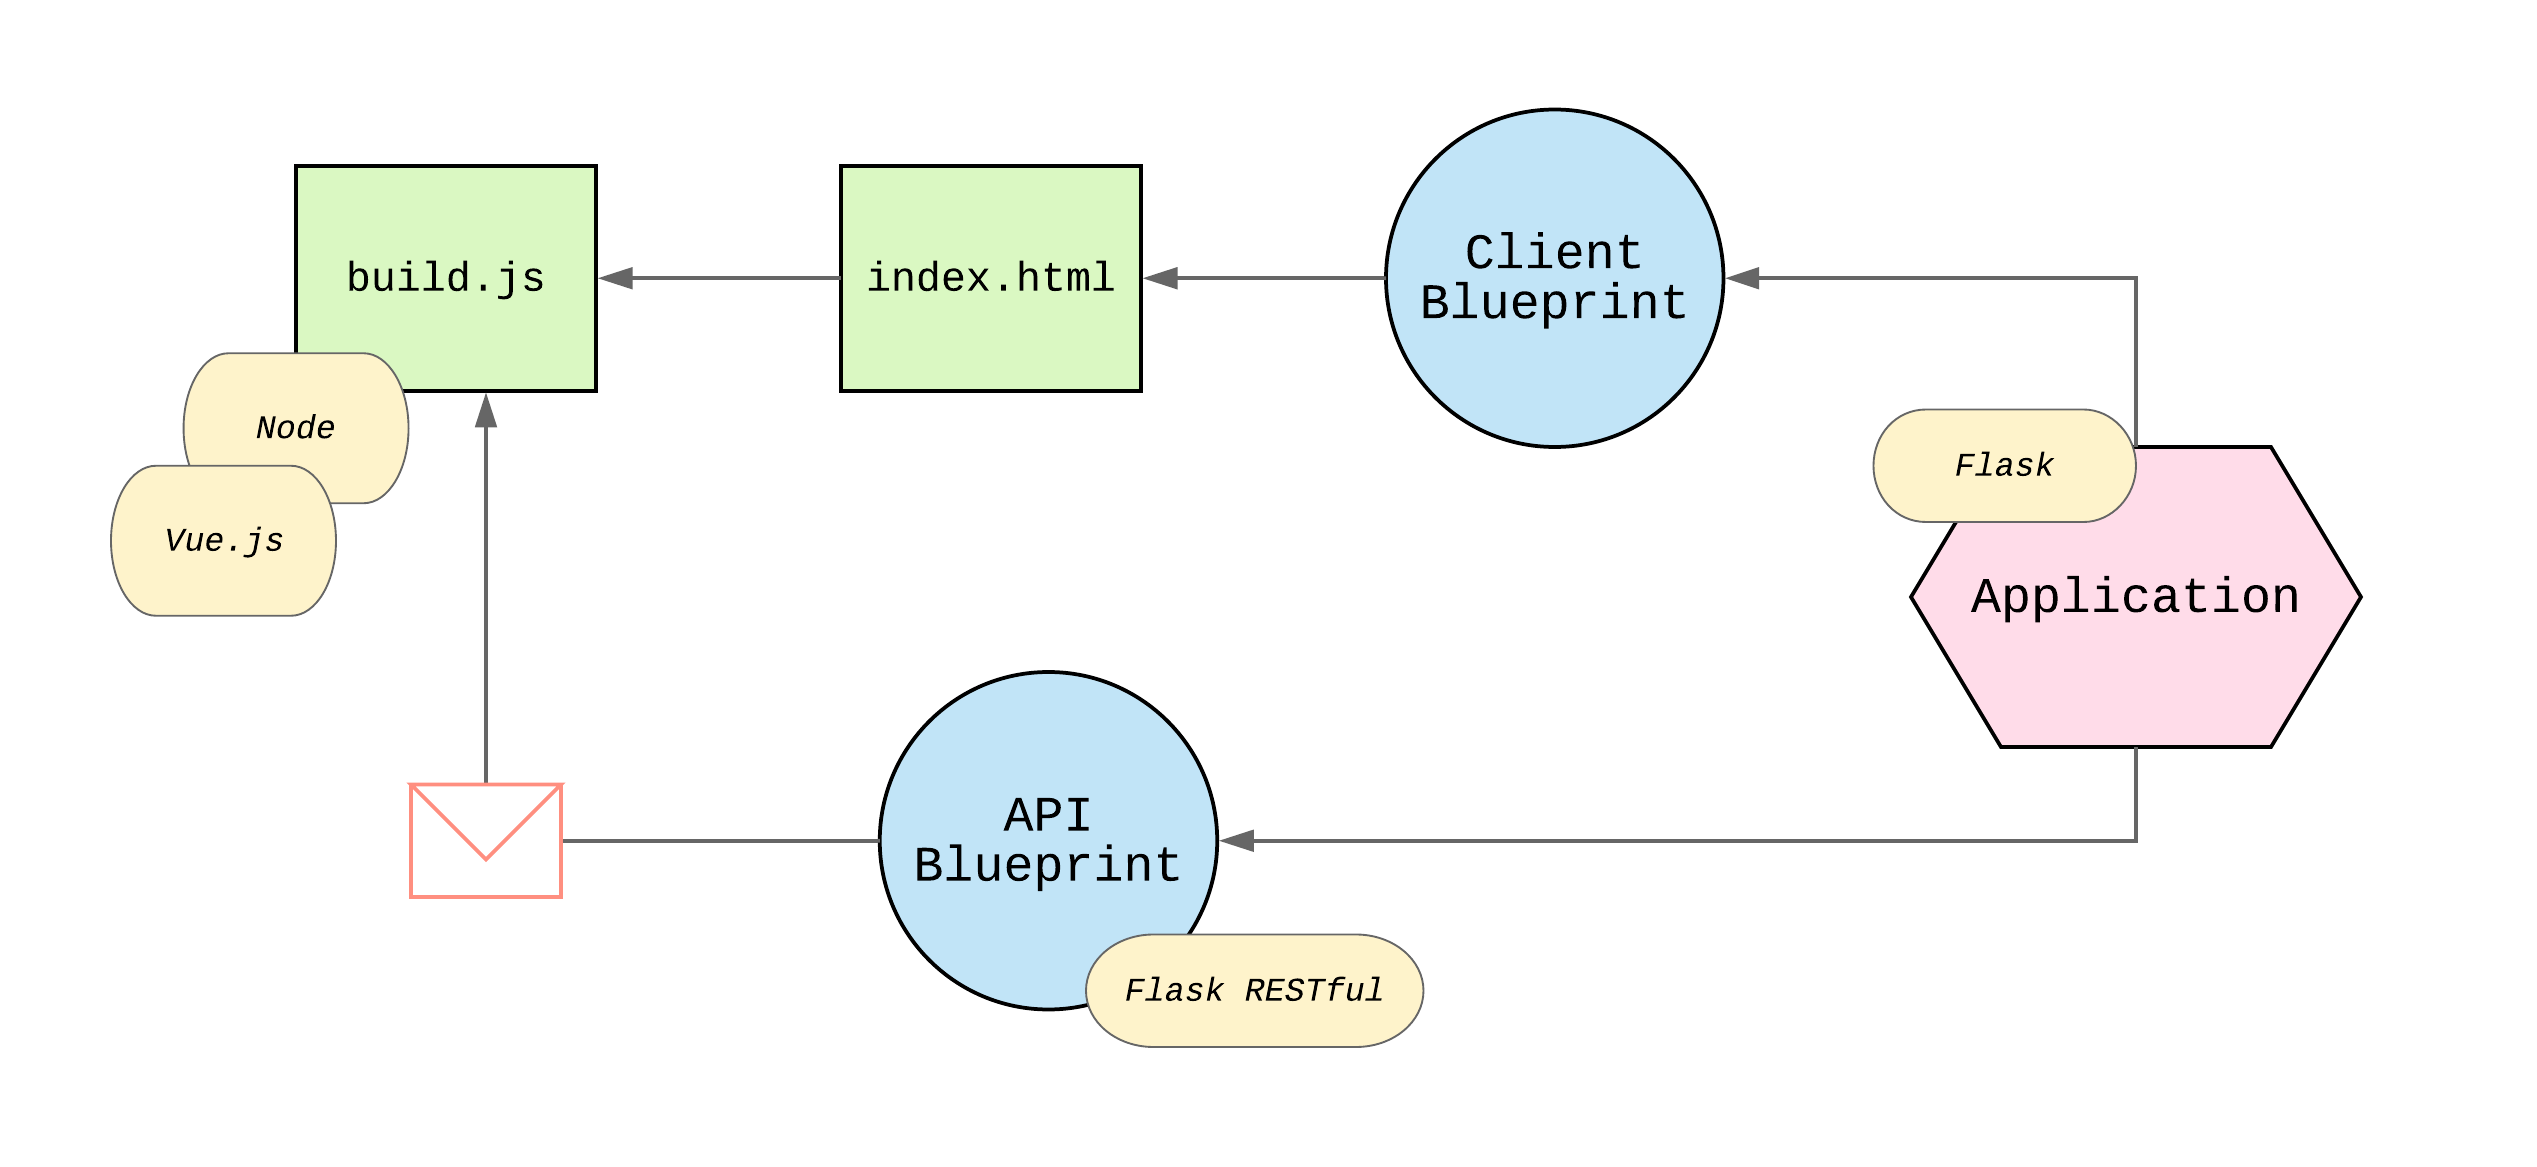
\includegraphics[width=0.9\textwidth, keepaspectratio]{img/techuml.png}
    \caption{Diagram of Application Design, \textit{April 2018}}
    \label{techuml}
\end{figure}

\subsection{Machine Learning}
The machine learning element of this application was built using Python 3 and TensorFlow. Machine learning is the use of statistics and computation in order to give systems the ability to "learn" and improve from past experience without being explicitly programmed to do so. Artificial neural networks, inspired by the biological networks within our brains, is the particular strain of machine learning which is used within this project.

The \textit{Long Short Term Memory} or LSTM algorithm, an efficient gradient-based model introduced by Hochreiter and Schmidhuber in 1997 \cite{lstm}, was used in the building of the neural network model for this system. \textit{Recurrent Neural Networks} attempt to address memory issues in traditional neural networks by adding loops within them, allowing information to persist \cite{colah}. A reasonable analogy, is to envision recurrent neural network as numerous copies of the same network, each passing a message to a parent. This chain-like nature resembles the behaviour of sequences and lists, making them naturally suited to the architecture of a neural network. 

Unfortunately, recurrent neural networks are burdened with the problem of handling long-term dependencies. As the neural network grows, gaps between past relevant data grows, and the recurrent neural network model becomes unable to learn to connect the information. In theory, recurrent neural networks are absolutely capable of handling this issue. In fact, some are. Long Short Term Memory is an extension or type of recurrent neural network that is capable, being very efficient on a large variety of problems including timeline data \cite{dashee}, and is now widely used to solve these problems. LSTM models have an additional loop learning what data to forget and what data to remember; they still have the aforementioned chain like structure, but with four different layers communicating in a certain way.


\subsubsection{Final Architecture}

In conclusion, the final architecture indeed differs somewhat from that which was originally planned. A diagram of the complete final architecture for the system is detailed below.
\\
\\
\\
\begin{figure}[h]
    \centering
    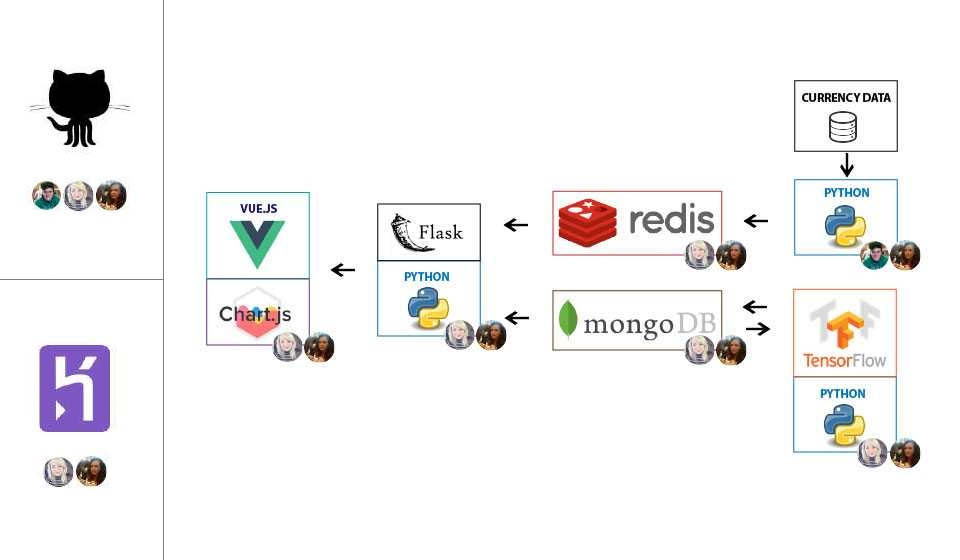
\includegraphics[width=0.9\textwidth, keepaspectratio]{img/newarchitecture.jpg}
    \caption{Final Architecture, \textit{April 2018}}
    \label{finalarchitecture}
\end{figure}